\chapter{Result}
\section{Pattern on Symmetry}\label{sec:pattsymm}
\subsection{Azimuthal Pattern}
Given in section \ref{sec:PCA}, there will be a particular pattern of nonzero singular values depending on the symmetry of the object. In the section \ref{subsec:azimsym}, it is explained that the azimuthal spherical harmonics components can be described by only one $m$ value for each $l$ or in other words only $m=0$ is nonzero. If the object has azimuthal symmetry then the matrix \Blq will only have one non zero significant singular value. 
\begin{figure}[ht]
  \centering
  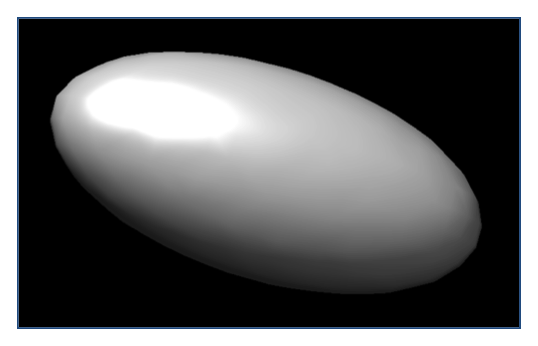
\includegraphics[width=.4\textwidth]{ellipsoid}
\caption{Model which has azimuthal symmetry}
\label{fig:ellipsoid}
\end{figure}

Figure \ref{fig:ellipsoid} is a model that is used to calculate \Blq. The model is ellipsoid which satisfy pure azimuthal symmetry, therefore \Blq inherently contain azimuthal symmetry. By taking SVD of the \Blq, the redundancy will be revealed and can be used to deduce the symmetry of object.
 \begin{figure}[ht]
  \centering
  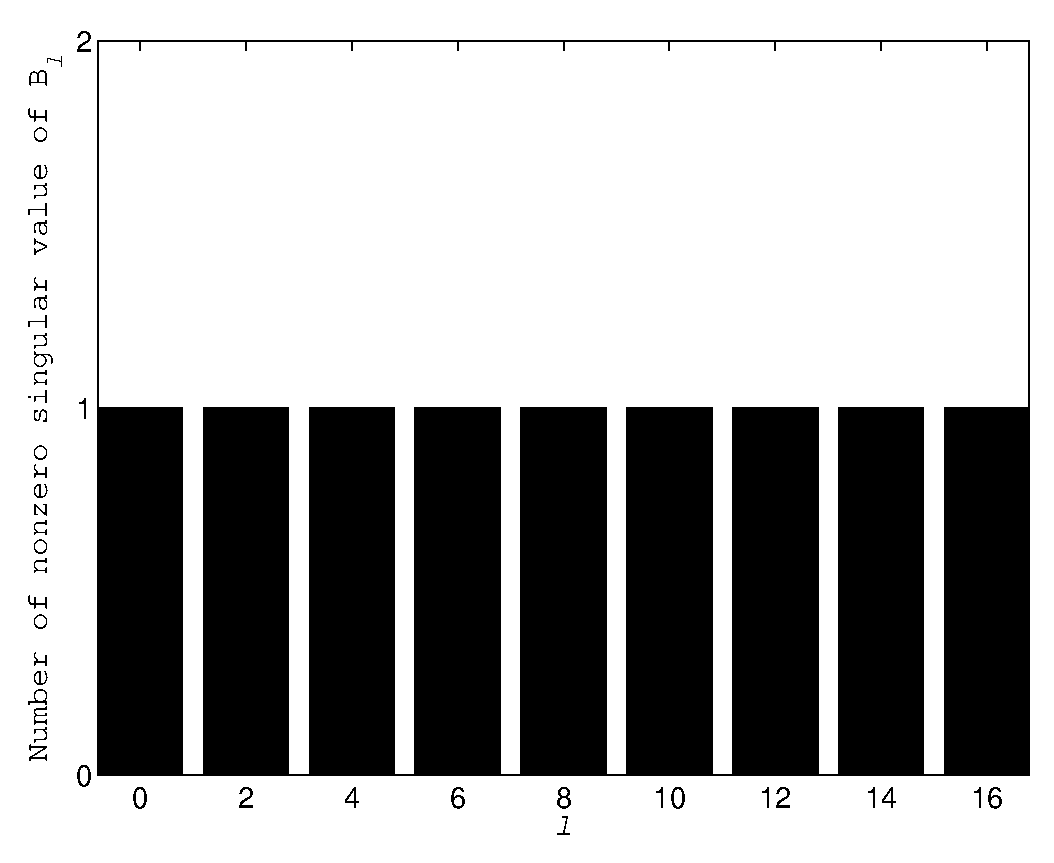
\includegraphics[width=.8\textwidth]{azimsvd}
\caption{Total number of nonzero singular values vs angular momentum}
\label{fig:azimsvd}
\end{figure}
\begin{figure}[ht]
  \centering
  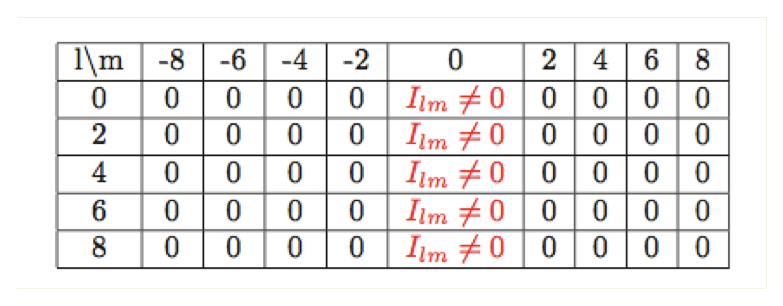
\includegraphics[width=.6\textwidth]{tableIlmazim}
\caption{Table of nonzero $I_{lm}$ for azimuthal symmetry}
\label{fig:azimtable}
\end{figure}

The graph on figure \ref{fig:azimsvd} shows the behavior of the singular value of the object which has azimuthal symmetry. It shows that only one nonzero singular value for each $l$, therefore it matchs the behavior of $I_{lm}$ which only $m=0$ is not vanish. Having said that, SVD of \Blq can be used to predict if the object satisfy azimuthal symmetry. 

\subsection{4-fold Pattern}
The example given here is for the object that has 4-fold symmetry. However in general it can be extended to any n-fold symmetry without losing of uniqueness. In the section \ref{subsec:fold4}, it is explained that if a 4-fold symmetry exist then the component of spherical harmonics, which the $l$'s are a multiple value of 4, will be nonzero. As consequence of that, the number of nonzero singular values of the matrix \Blq has pattern that match with the total number of nonzero components in spherical harmonics expansion.  

\begin{figure}[ht]
  \centering
  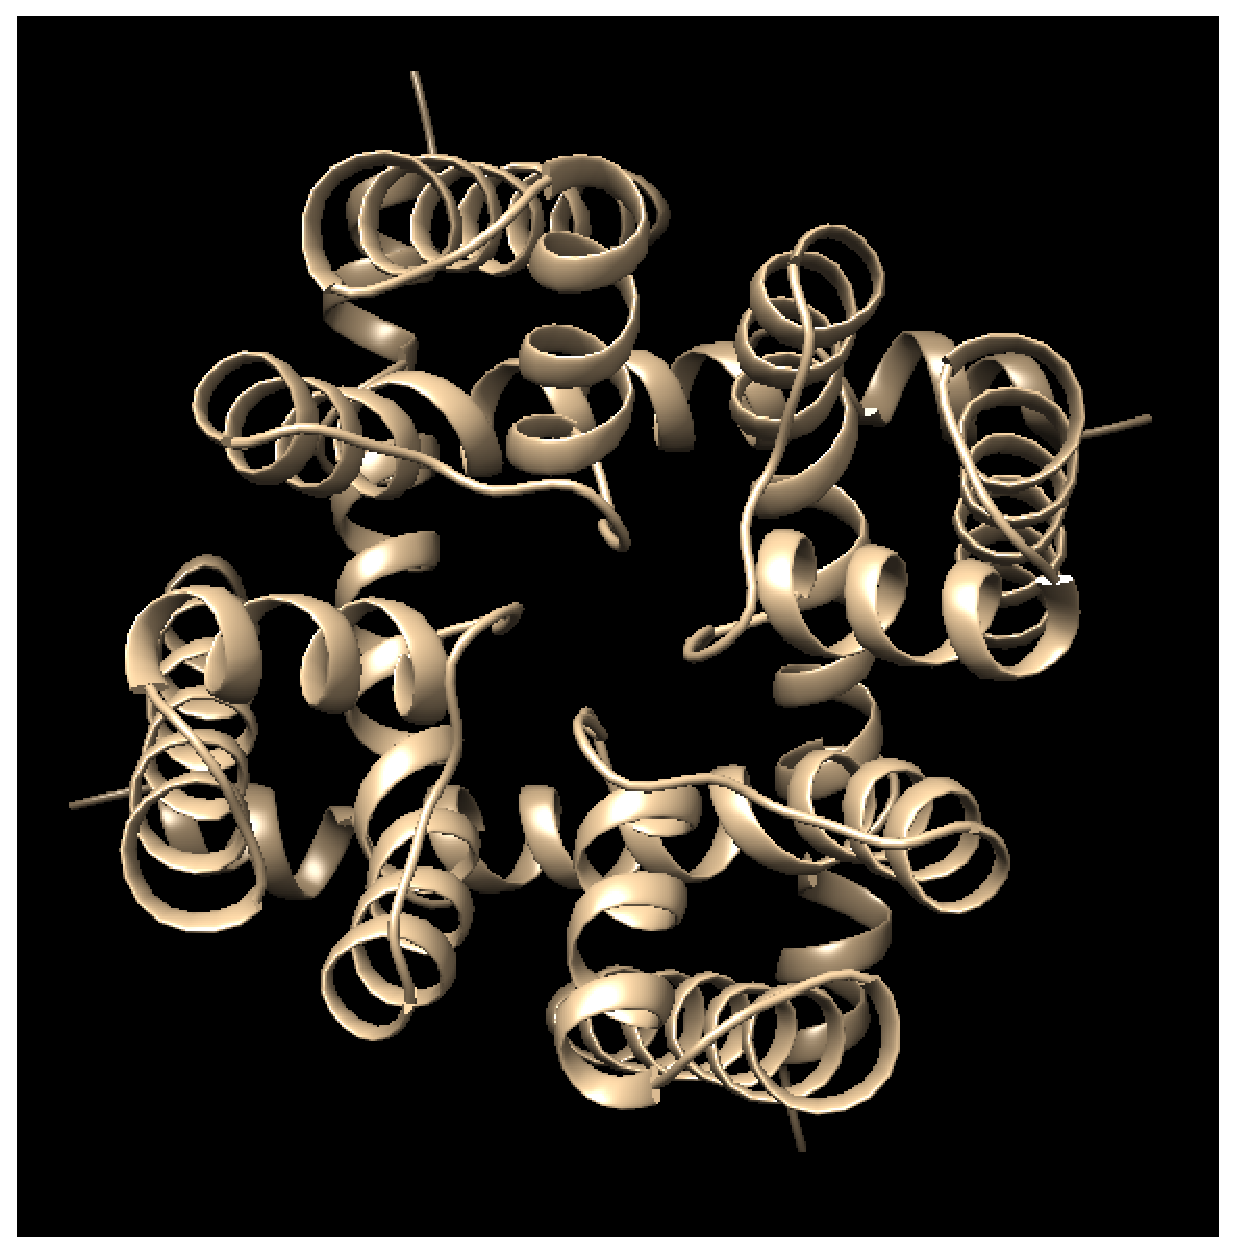
\includegraphics[width=.6\textwidth]{KC4fold}
\caption{K-channel protein has 4-fold symmetry}
\label{fig:KC4fold}
\end{figure}

The figure \ref{fig:KC4fold} shows 4-fold symmetric model that is used to calculate \Blq. 
Because the model has 4-fold symmetry, the \Blq inherently contain information about the 4-fold symmetry. 
By taking SVD of the \Blq, the redundancy will be revealed and can be used to deduce the symmetry of object. From figure \ref{fig:4foldsvd} and table \ref{fig:4foldtable}, there is a matching pattern. By comparing them, for $l=2$ there is one nonzero singular value and there is only one nonzero $I_{lm}$ that is when $m=0$. 
Another example is for $l=6$, there are 4 singular value from figure  \ref{fig:4foldsvd} and from table \ref{fig:4foldtable} there are 3 nonzero $I_{lm}$ that is when $m=-4,0,4$. If unknown structure give the same behavior as in graph \ref{fig:4foldsvd} then one can conclude it has 4-fold symmetry. 
\begin{figure}[h]
  \centering
  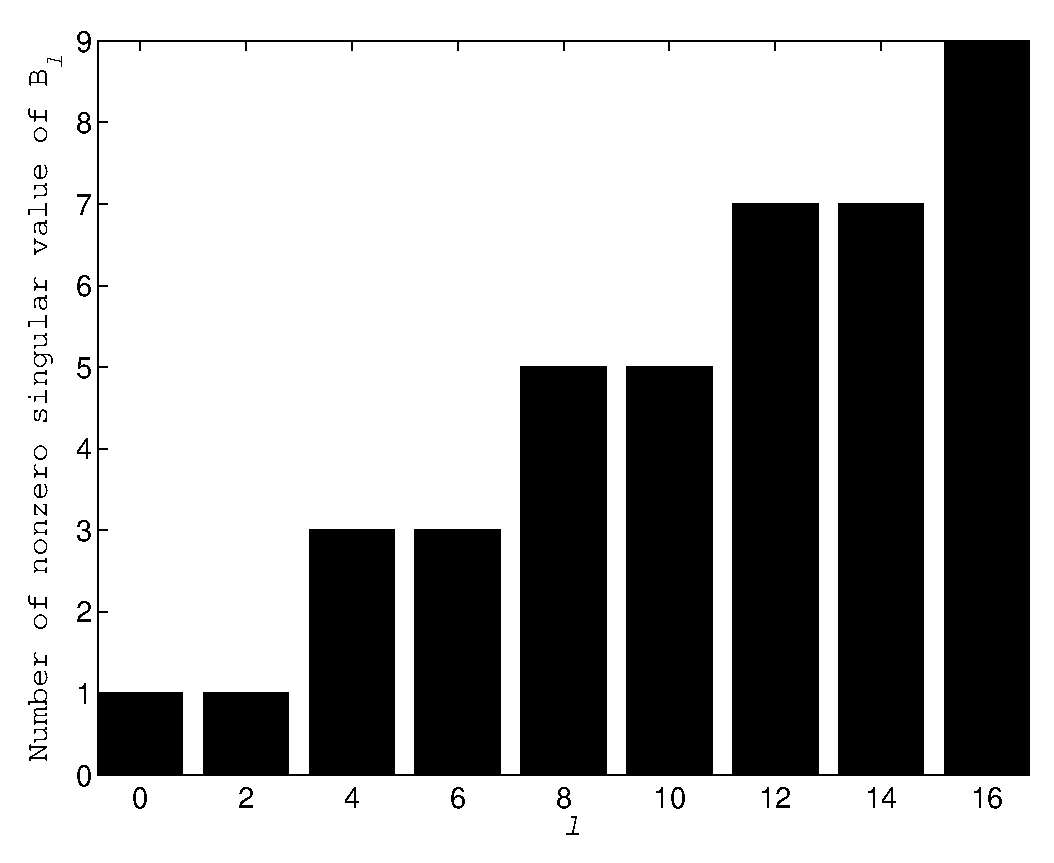
\includegraphics[width=.8\textwidth]{svdKC}
\caption{Total number of nonzero singular values vs angular momentum}
\label{fig:4foldsvd}
\end{figure}
\begin{figure}[ht]
  \centering
  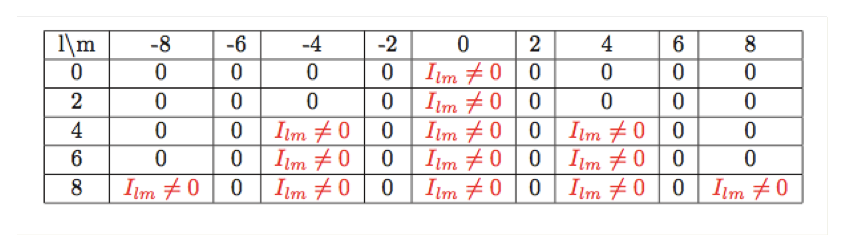
\includegraphics[width=.6\textwidth]{tableIlm4fold}
\caption{Table of nonzero $I_{lm}$ for 4-fold symmetry}
\label{fig:4foldtable}
\end{figure}

\subsection{Icosahedral Pattern}
One of the important symmetry to be demonstrated in this section is icosahedral symmetry. Previous section explains that there is only one singular value of \Blq if the object has icosahedral symmetry.
 In addition to that, there is a selection rule of $l$'s for icosahedral harmonics. In order to predict the icosahedral symmetry both the selection rule and the singular value has to be satisfied. 
\begin{figure}[h!]
  \centering
  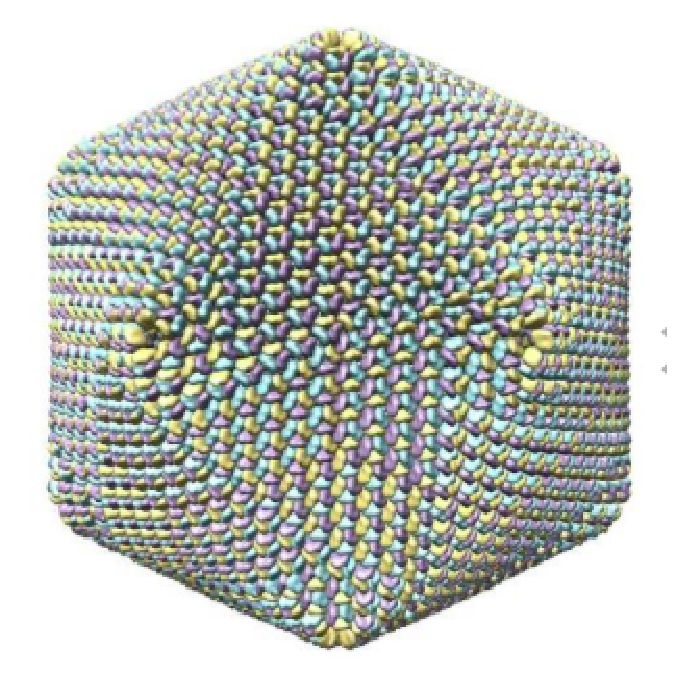
\includegraphics[width=.5\textwidth]{cor}
\caption{PBCV from pdb(1m4x) is used as model that has icosahedral symmetry \cite{pdb1m4x}}
\label{fig:icopbcv}
\end{figure}

The figure \ref{fig:icopbcv} is model that is used to calculate \Blq. The model is a virus that satisfy pure icosahedral symmetry. Thus, \Blq inherently contain the icosahedral symmetry. By taking SVD of \Blq, the redundancy will be revealed and can be used to deduce the symmetry of the object.
\begin{figure}[h!]
  \centering
  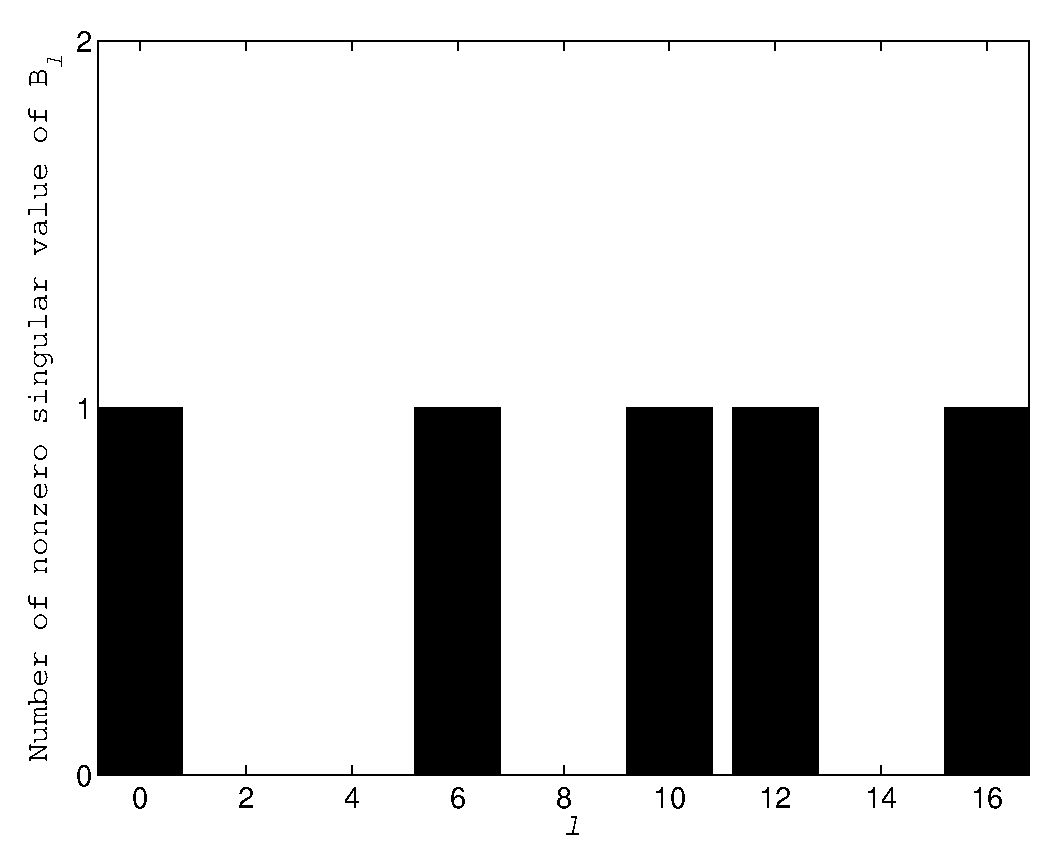
\includegraphics[width=.8\textwidth]{svdBcor}
\caption{Total number of nonzero singular values vs angular momentum}
\label{fig:svdico}
\end{figure}

The figure \ref{fig:svdico} is a graph calculated from svd of \Blq. It is obviously seen that it follows icosahedral selection rule and at the same time has one singular value for each $l$. If unknown structure give behavior as in graph \ref{fig:svdico} then one can conclude it has icosahedral symmetry.   
\subsection{Asymmetric Pattern}
In this section distinguishing  asymmetric property is demonstrated. Previous section explains that there will be $2l+1$ singular value if the object under study has asymmetric property. The number of singular values is equal to total component in spherical harmonics expansion. 
\begin{figure}[h!]
  \centering
  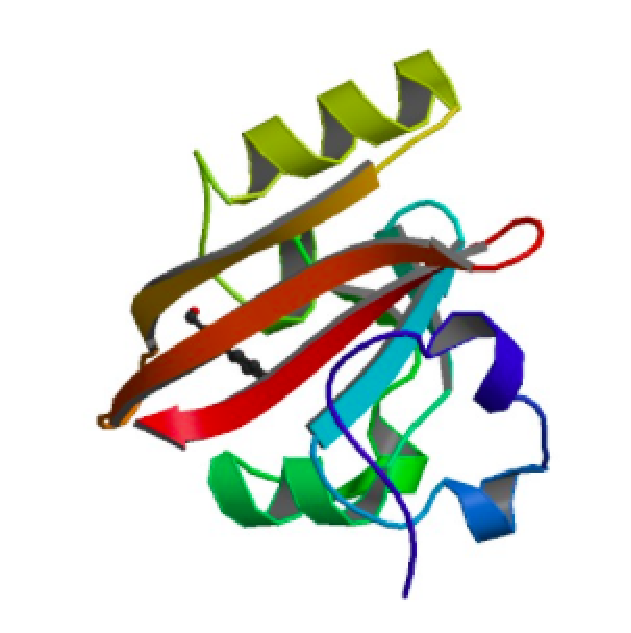
\includegraphics[width=.5\textwidth]{pyp}
\caption{Photoactive yellow protein from pdb(2phy) is used as model}
\label{fig:pyp}
\end{figure}

The figure \ref{fig:pyp} is a model that is used to calculate \Blq. The model is pyp protein, which doesn't have symmetry at all, therefore \Blq inherently contain asymmetric property. From figure \ref{fig:svdPYP}, for every $l$'s there are $2L+1$ singular values. As already mentioned before, $2l+1$ singular values represent asymmetric pattern. If an unknown structure give a behavior as in graph \ref{fig:svdPYP} then one can conclude that it has asymmetry property.   
\begin{figure}[h!]
  \centering
  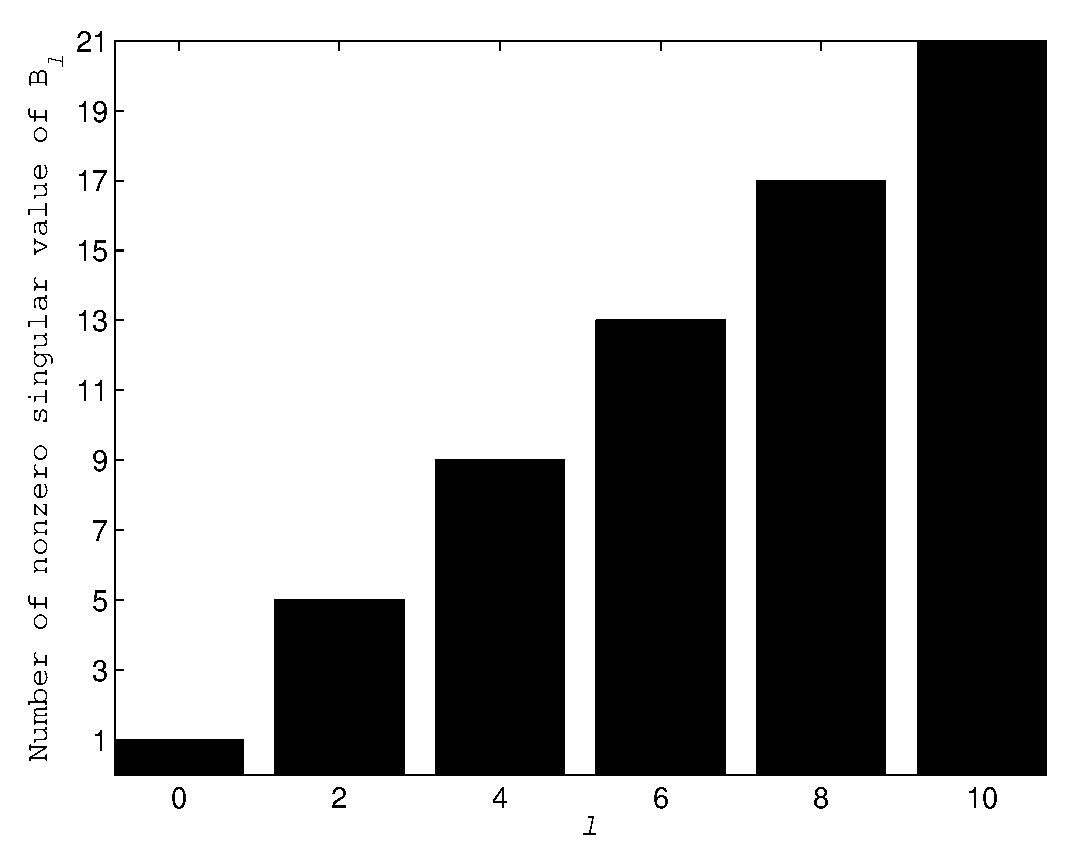
\includegraphics[width=.8\textwidth]{svdBaPYP}
\caption{Total number of nonzero singular values vs angular momentum}
\label{fig:svdPYP}
\end{figure}

This asymmetric pattern can be used to inspect whether \Blq is a form of a dot product. Because no shape can be more asymmetrical than asymmetric shape, no shape can have more number of singular values than an asymmetric shape. In other words, $2l+1$ is the highest number of singular values and all shapes should have number of singular values less than or equal $2l+1$. If an SVD on the \Blq has more singular values than $2l+1$ then the \Blq is not a form of dot product or convergence is not reached.  


\subsection{Inversion Symmetry}
This section describes one of the limits of the methods (PCA and selection rule) by giving an analysis of applying inversion symmetry. Because the available data from the experiment is a collection of diffraction patterns, all analyses initially have to be done in reciprocal space. It applies also to the determination of symmetry because the actual symmetry being determined is the symmetry of the diffraction volume. The symmetry of the structure is deduced from the symmetry of the diffraction volume because their relation is Fourier transform and an operation of Fourier transform preserves the symmetry. As a result of that, PCA and the selection rule are used to determine the symmetry of the molecule implicitly through the determination of the symmetry in the diffraction volume.

If a molecule has inversion symmetry then each atom can be moved along inversion center to a point of equal distance without changing the whole shape of the molecule. The operation of inversion symmetry is changing each point $(x,y,z)$ to $(-x,-y,-z)$ where $(0,0)$ is the inversion center. Any function that has inversion symmetry is invariant under the operation of inversion symmetry.  Mathematically, it is described as
\begin{equation}
f(x,y,z)=f(-x,-y,-z). 
\label{eq:invfunc}
\end{equation}

Spherical harmonics has a distinct property to reveal the existence of inversion symmetry in a function. The analysis comes from the property of spherical harmonics where it is multiplication between exponential and Legendre polynomial. The inversion symmetry in polar coordinate is by tranforming $\theta \rightarrow \pi-\theta$ and $\phi \rightarrow \phi+\pi$. Mathematically, under the invariance of inversion symmetry from equation \ref{eq:invfunc}, spherical harmonics follow this property where
\begin{align}
\begin{split}
Y_{lm}(\theta,\phi)&=Y(\pi-\theta,\phi+\pi) \\
&\propto P_{lm}(\cos(\pi-\theta)) \exp(i m (\phi+\pi)) \\
&\propto  (-1)^{m+l} P_{lm}(\cos(\theta)) (-1)^m \exp(i m (\phi)) \\
&\propto  (-1)^{l} Y_{lm}(\theta,\phi) \\
\end{split}
\label{eq:sphinver}
\end{align}

The expression in equation \ref{eq:sphinver} always hold true for all components. Similarly, the spherical harmonics expansion ($I_{lm}(q)$) also follow the relation in equation \ref{eq:sphinver}. From equation \ref{eq:sphinver}, it is obvious that if the original function has inversion symmetry then its spherical harmonics expansion are zero for odd $l$ and non-zero for even $l$. 

In the previous discussion of symmetry, only even $l$ are shown because all odd $l$ are equal to zero. In other words, even though the original model doesn’t have inversion symmetry but their \Ilm has the inversion symmetry (the \Ilm is defined as spherical harmonics expansion of a diffraction volume). The diffraction volume is an absolute square of a structure factor, in which the structure factor is the result of a Fourier transfom of an electron density. Because the electron density is a quantity, which is described by real number, the following relation hold true:
\begin{align}
A(\vec{q})&=\int \rho(\vec{r}) \exp(2 \pi i \vec{q} \cdot \vec{r}) \nonumber \\
A^{*}(\vec{q})&=\int \rho(\vec{r})^{*} \exp(-2 \pi i \vec{q} \cdot \vec{r}) \nonumber\\
A^{*}(\vec{q})&=\int \rho(\vec{r}) \exp(-2 \pi i \vec{q} \cdot \vec{r}) \nonumber\\
A^{*}(-\vec{q})&= A(\vec{q}) \nonumber\\
|A^{*}(-\vec{q})|^{2}&= |A(\vec{q})|^2 \nonumber\\
I(-\vec{q})&= I(\vec{q}). 
\label{eq:ftinv}
\end{align}
The relation is called Friedel's law. In other words, all diffraction volume will always have inversion symmetry even though the electron density doesn’t have inversion symmetry.

In conclusion, the inversion symmetry cannot be distinguished by using PCA nor by using selection rule. Another key point is that all electron density are described by real numbers (not complex numbers) and always have inversion symmetry in its diffraction volume regardless of whether the original electron density has inversion symmetry or not. By knowing only the diffraction volume, it is not sufficient to deduce if there is such symmetry in the electron density, therefore the inversion symmetry cannot be determined by the method explained above.

\subsection{Experimental Data}
This section mainly explains how to calculate \Blq from experiment data and the convergence of \Blq. For this reason, the experiment diffraction patterns of nanorice were used to calculate \Blq. The diffraction patterns are available online and can be downloaded from cxidb.org.

\begin{figure}[ht]
\begin{subfigure}{.5\textwidth}
  \centering
  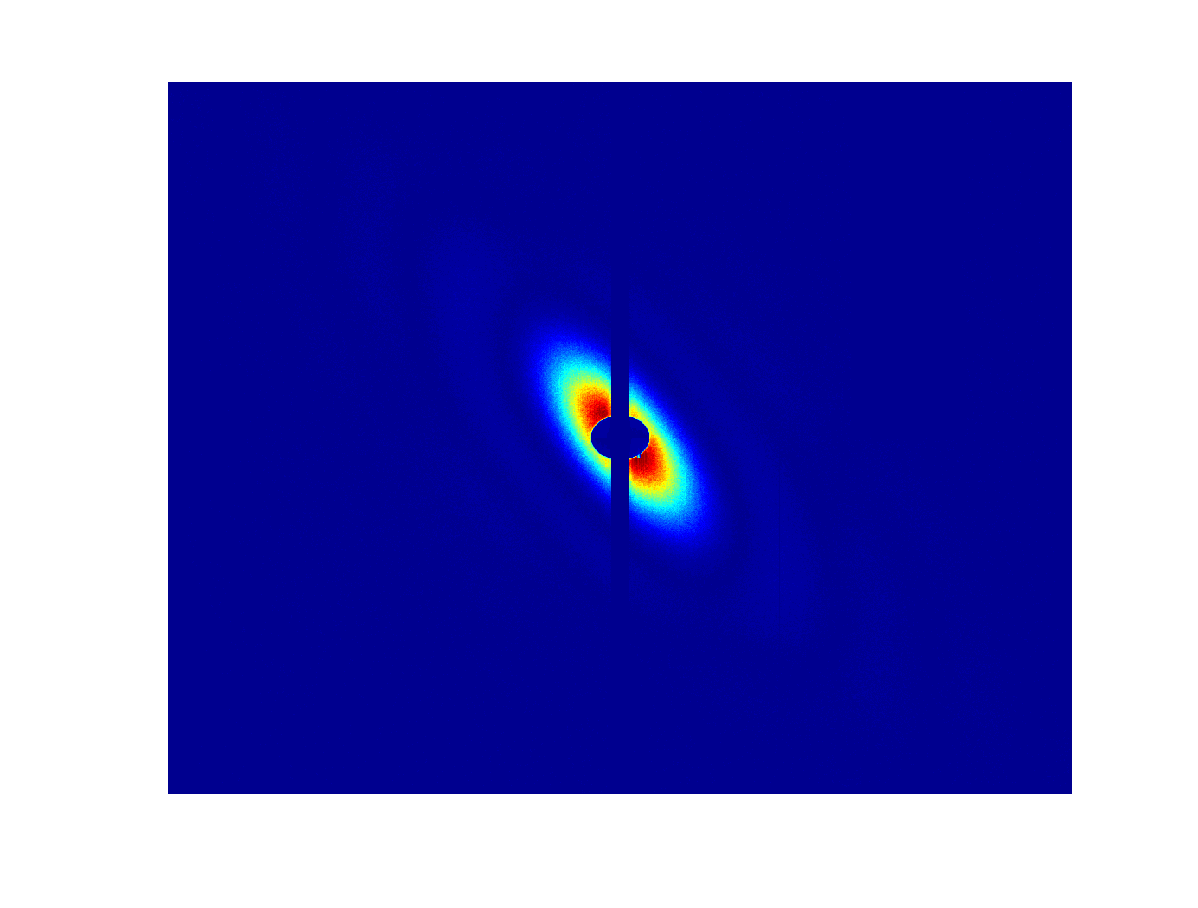
\includegraphics[width=.8\textwidth]{good1}
\end{subfigure}
\begin{subfigure}{.5\textwidth}
  \centering
  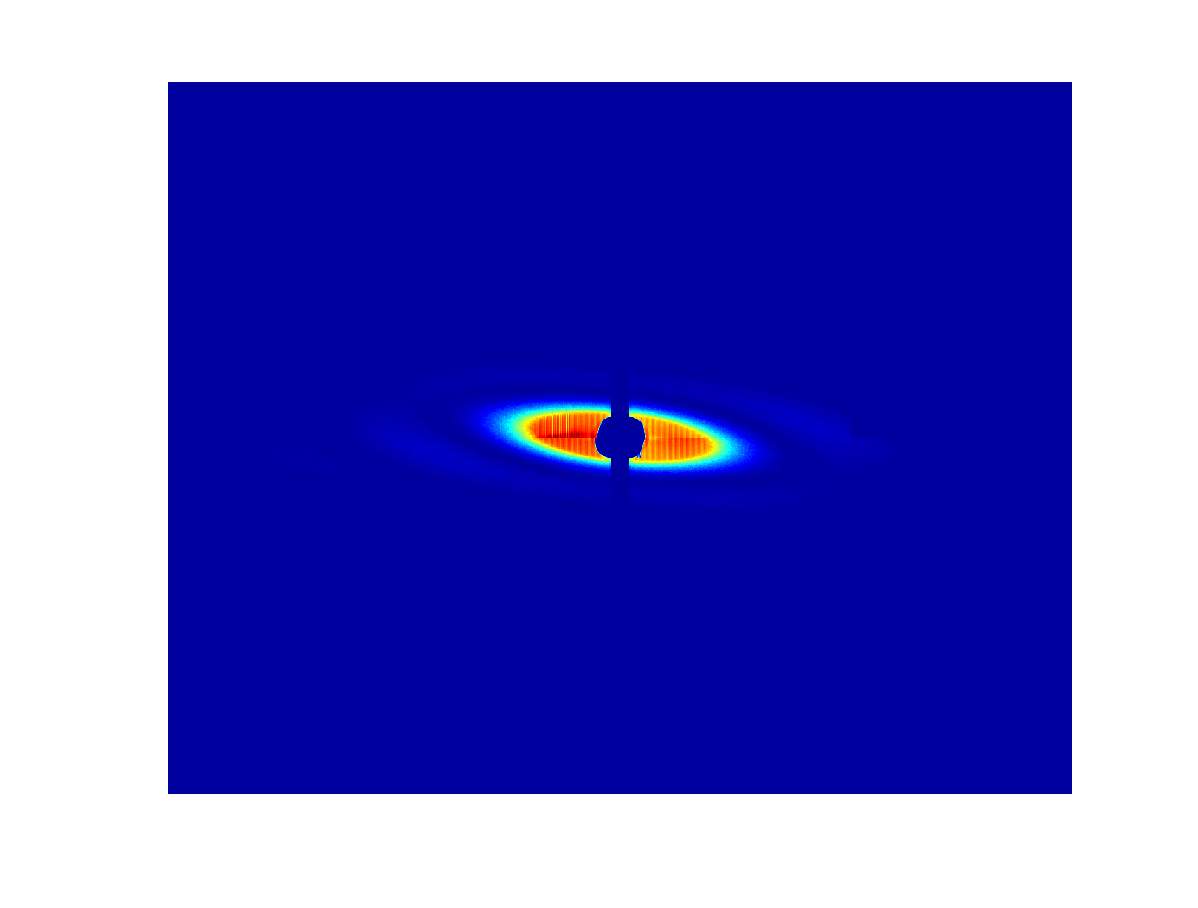
\includegraphics[width=.8\textwidth]{good2}
\end{subfigure}
\begin{subfigure}{.5\textwidth}
  \centering
  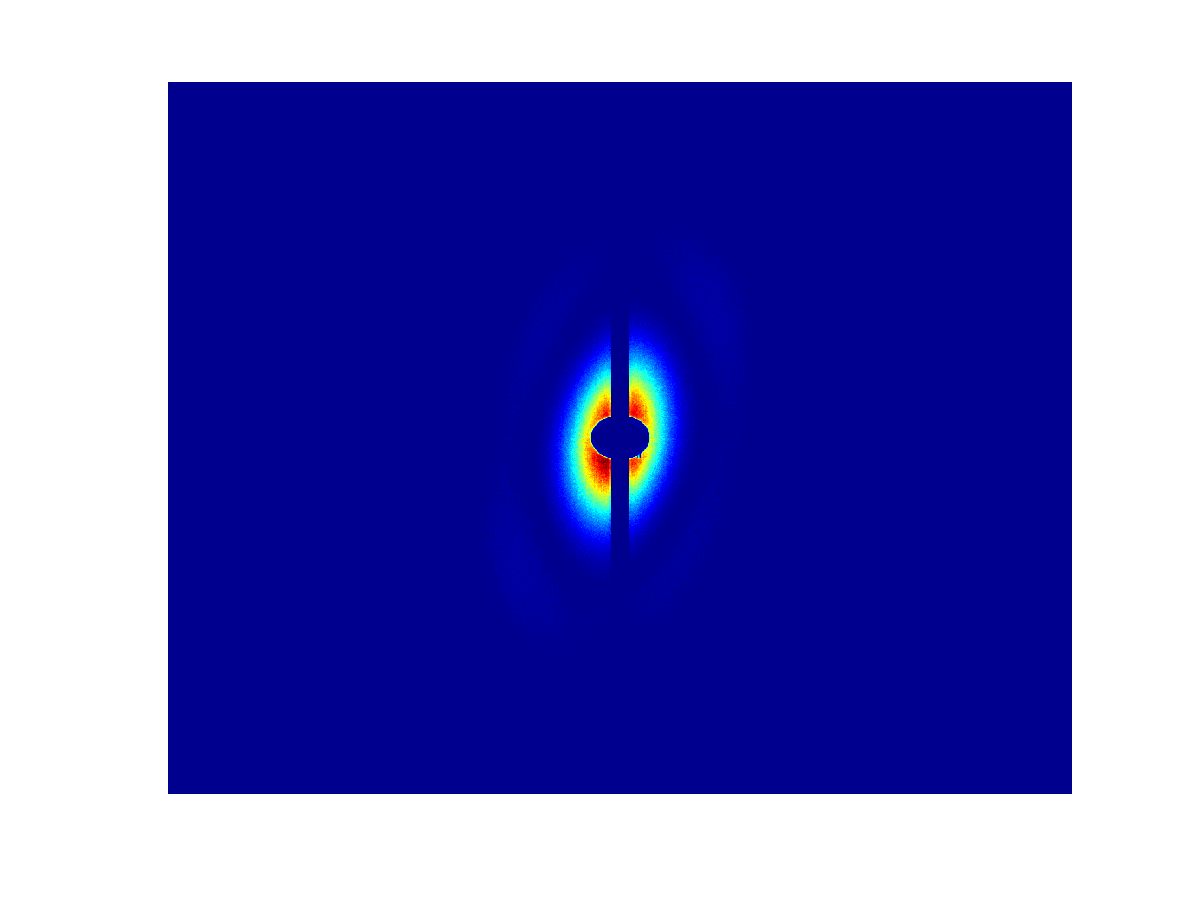
\includegraphics[width=.8\textwidth]{good3}
\end{subfigure}
\begin{subfigure}{.5\textwidth}
  \centering
  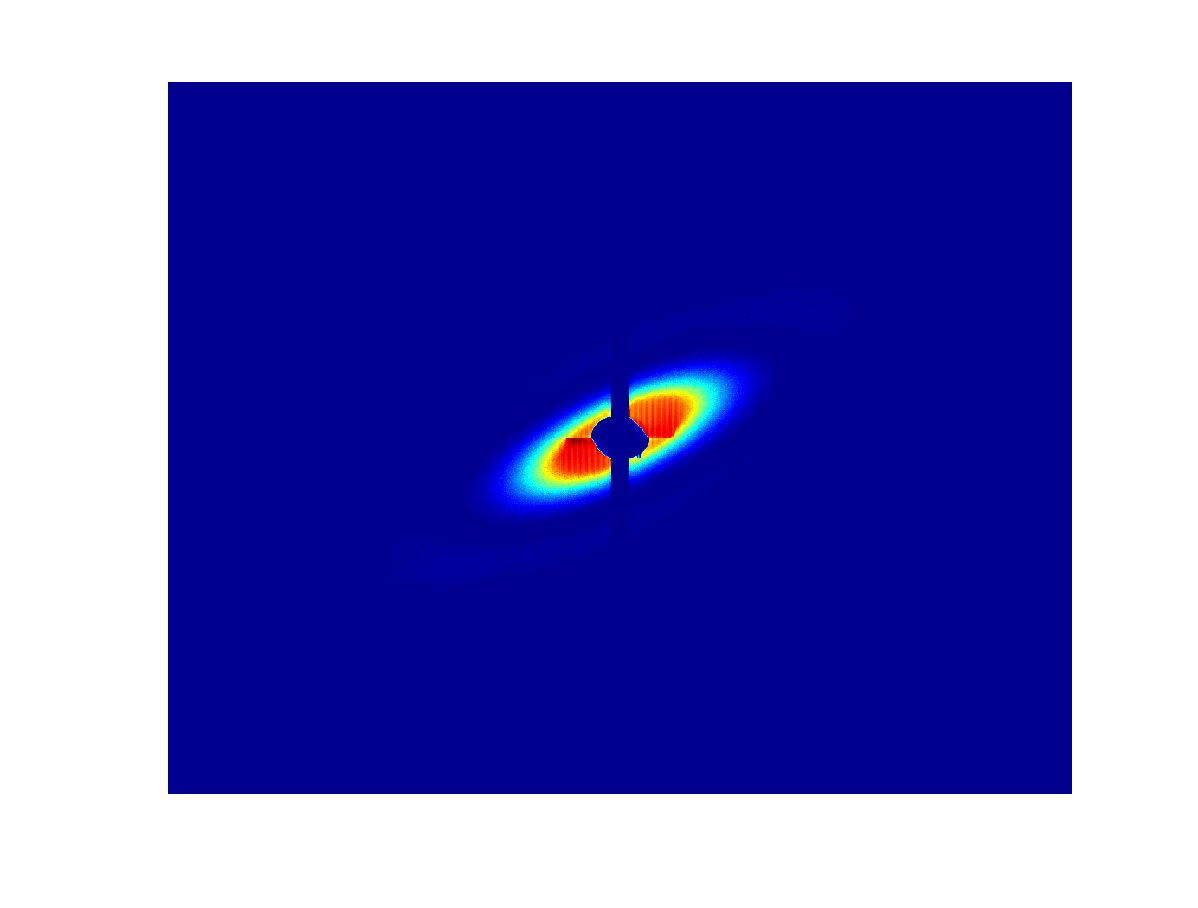
\includegraphics[width=.8\textwidth]{good4}
\end{subfigure}
\caption{Diffraction pattern that are considered as "good"}
\label{fig:gooddp1}
\end{figure}

The initial step that I did to analysis the experiment data was to separate good data from bad data. Figure \ref{fig:gooddp1} are some examples of the good data. Because it is known that the molecule is nanorice, it is expected to be close to ellipsoid. In addition to that, the diffraction patterns of ellipsoid can be easily identified. Thus, those several patterns in figure \ref{fig:gooddp1} shows the behavior where the diffracted molecules have the ellipsoidal property. Currently, by checking the data visually, I collected 200 good diffraction patterns.

\begin{figure}[ht]
\begin{subfigure}{.5\textwidth}
  \centering
  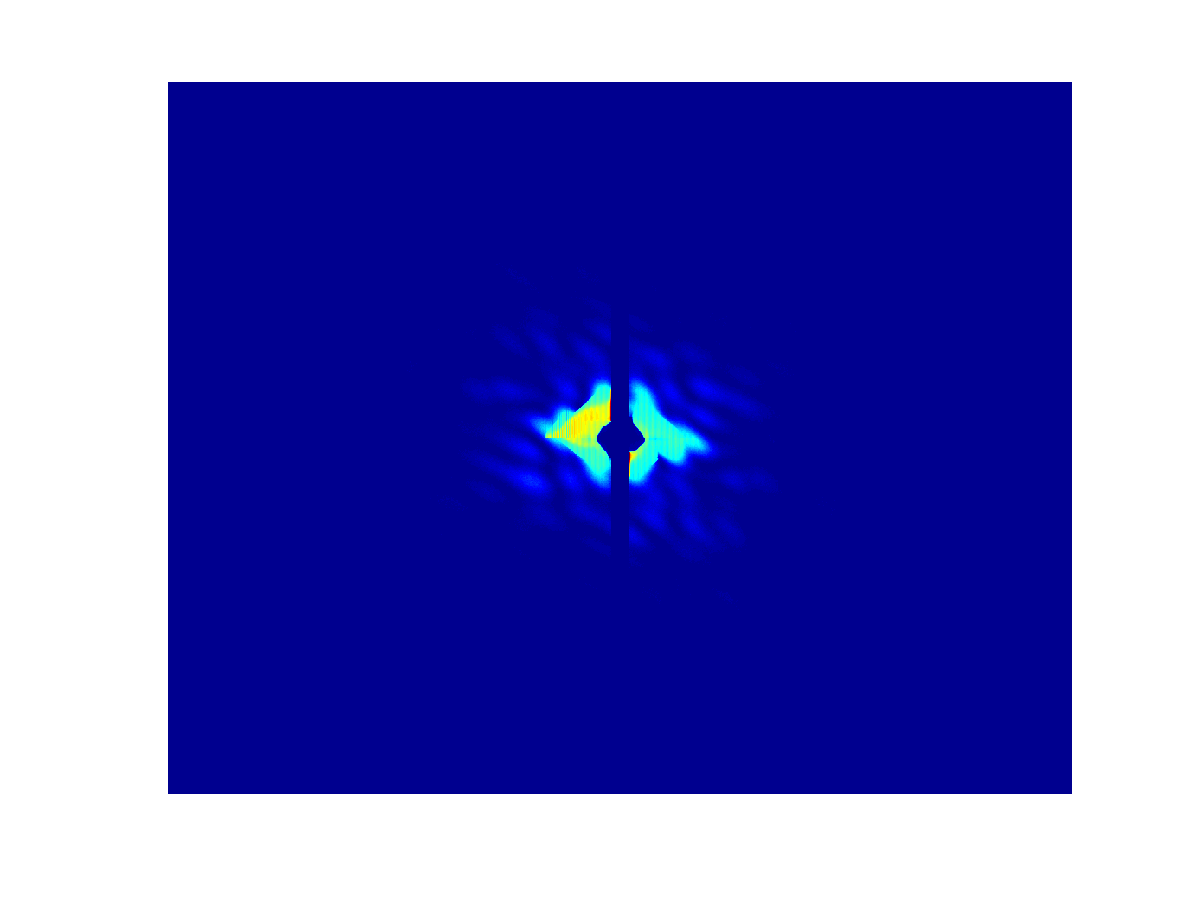
\includegraphics[width=.8\textwidth]{bad1}
\end{subfigure}
\begin{subfigure}{.5\textwidth}
  \centering
  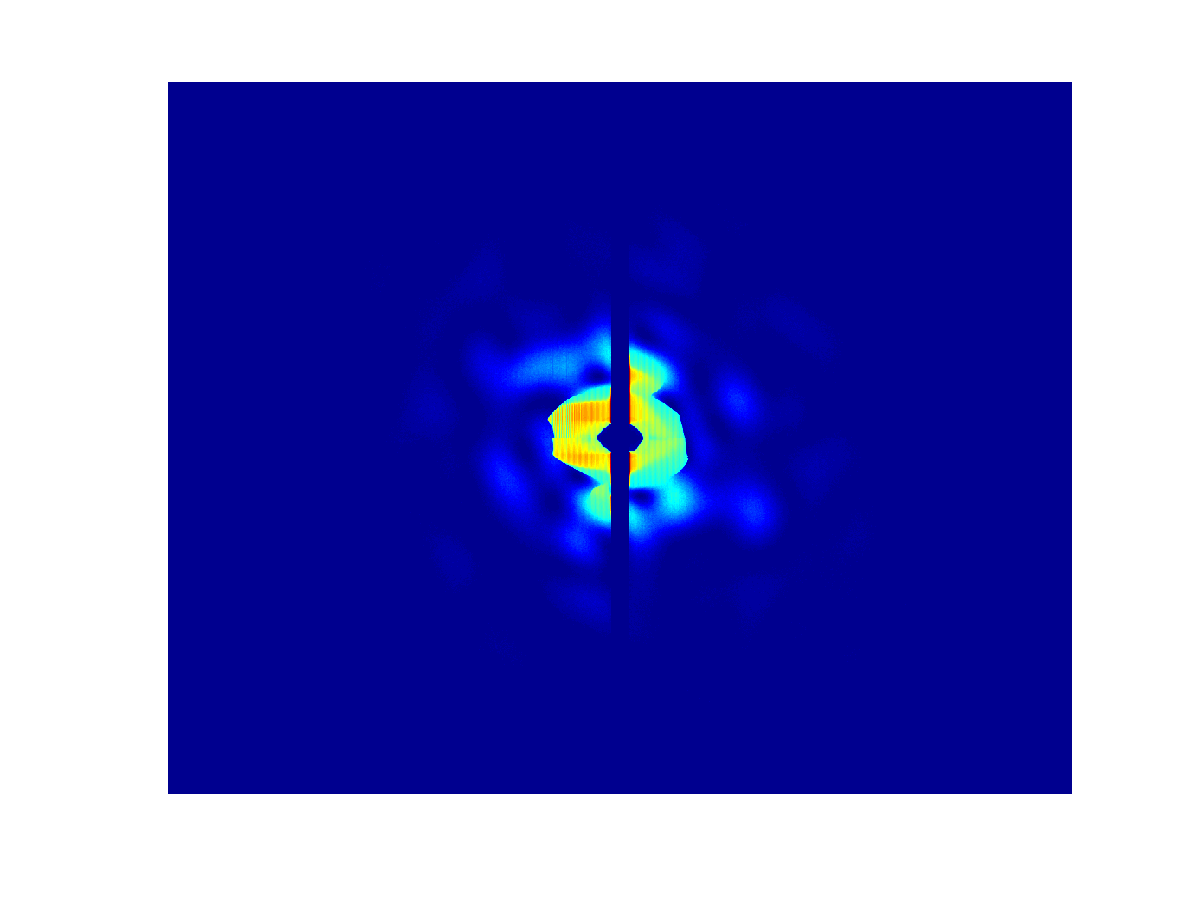
\includegraphics[width=.8\textwidth]{bad2}
\end{subfigure}
\begin{subfigure}{.5\textwidth}
  \centering
  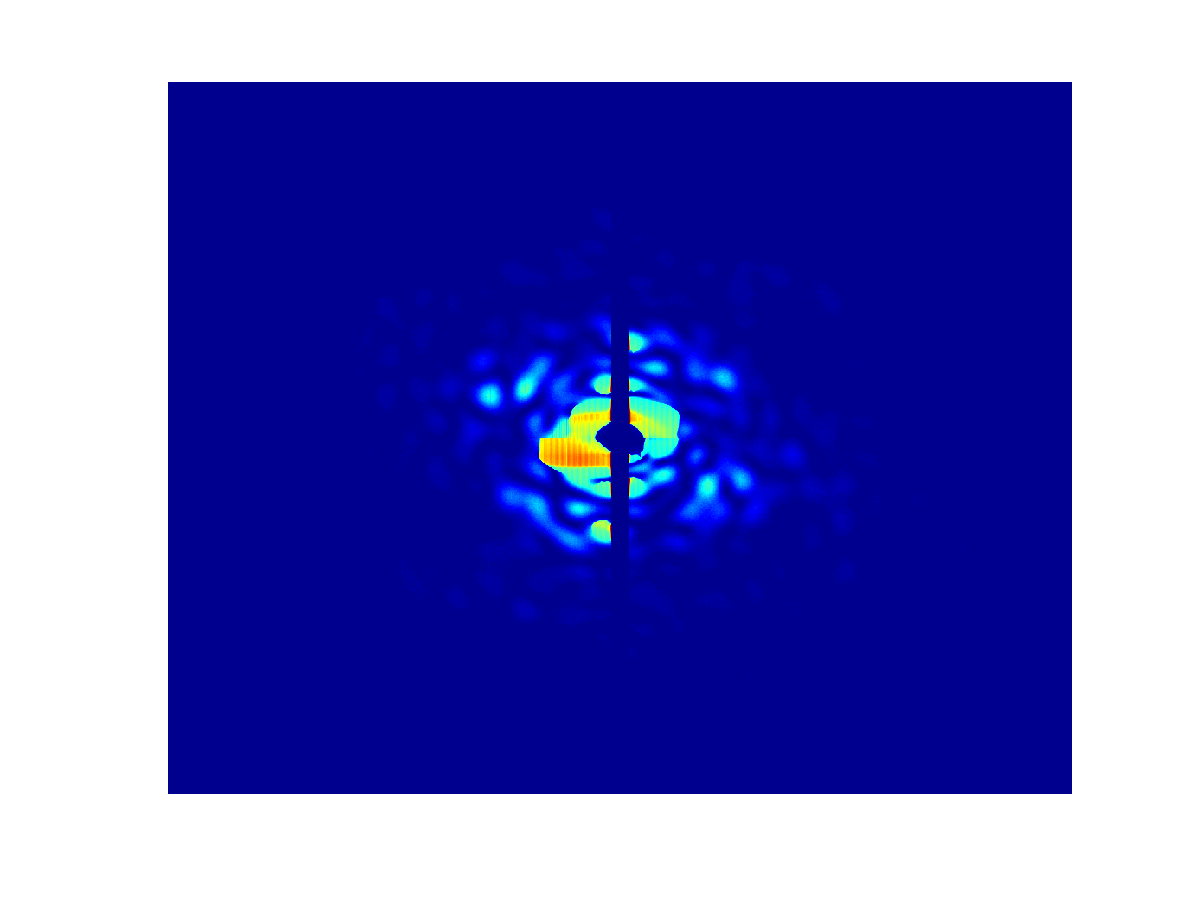
\includegraphics[width=.8\textwidth]{bad3}
\end{subfigure}
\begin{subfigure}{.5\textwidth}
  \centering
  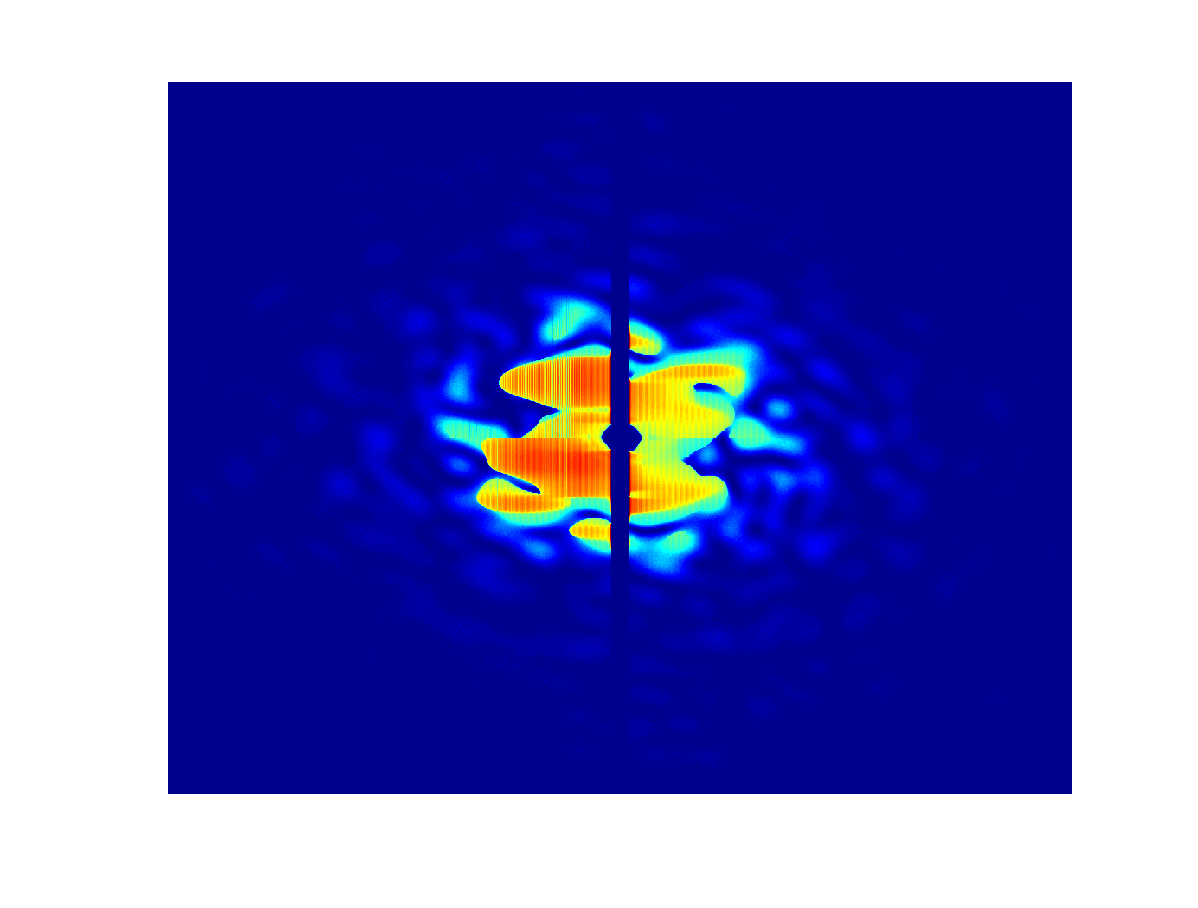
\includegraphics[width=.8\textwidth]{bad4}
\end{subfigure}
\caption{Diffraction patterns that are considered as "bad"}
\label{fig:baddp1}
\end{figure}

The exclusion bad data is simpler than finding a good one. If the diffraction patterns doesn't contain signal then they are bad data. Several example of diffraction patterns that doesn't contain strong signal is given in figure \ref{fig:baddp2}. Beside that, there is another type of bad data where the diffraction pattern doesn't seem to have ellipsoidal symmetry. Typical of those diffraction patterns are is displayed in figure \ref{fig:baddp1}. Because the nanorice in general is simple structure (close to ellipsoid), it is expected its diffraction pattern to be close to ellipsoid diffraction pattern. Thus, the diffraction pattern in figure \ref{fig:baddp1} doesn't come from the nanorice and need to be excluded for the calculation of \Blq. Given the current stage of algorithm, the algorithm need to impose azimuthal symmetry then such diffraction patterns, which doesn't show the ellipsoidal behavior, cannot be used to recover electron density. 
\begin{figure}[h]
\begin{subfigure}{.5\textwidth}
  \centering
  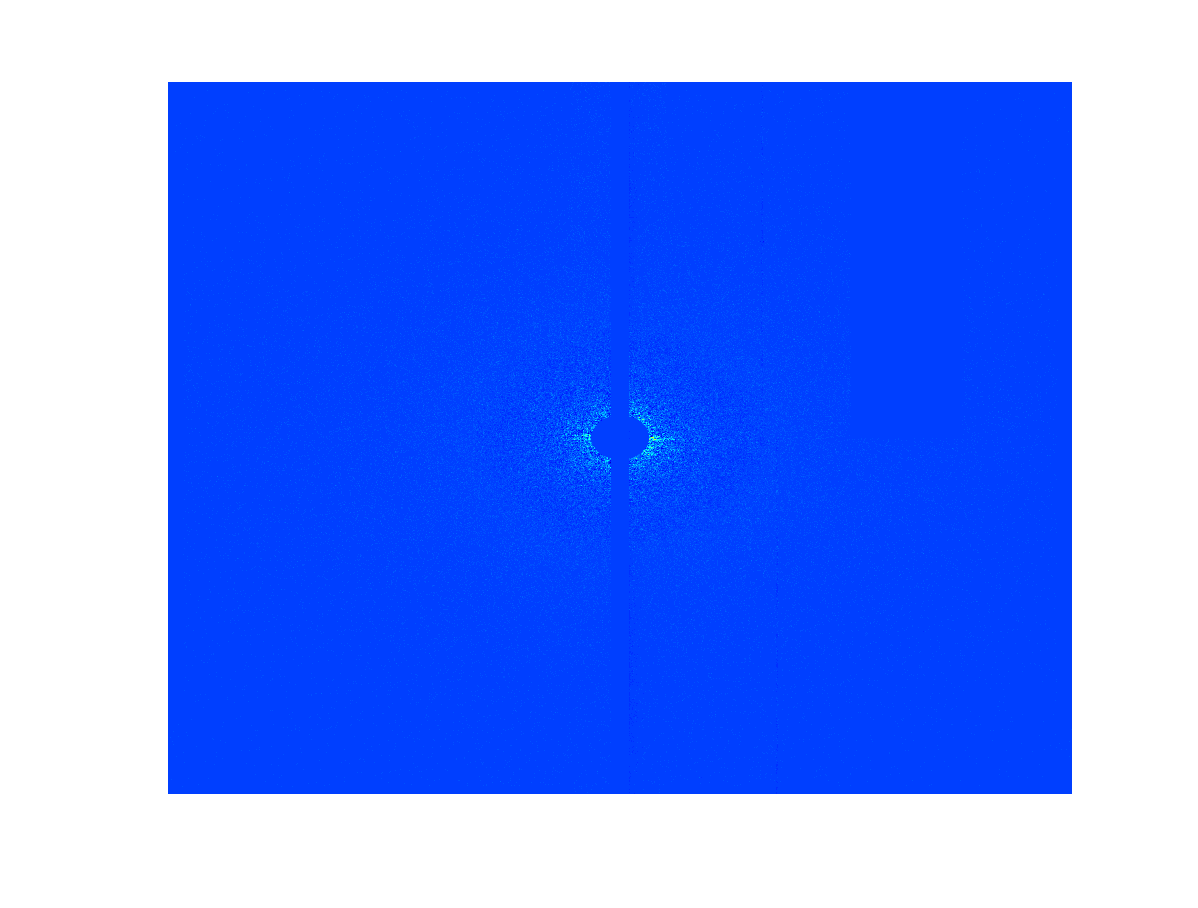
\includegraphics[width=.8\textwidth]{bad5}
\end{subfigure}
\begin{subfigure}{.5\textwidth}
  \centering
  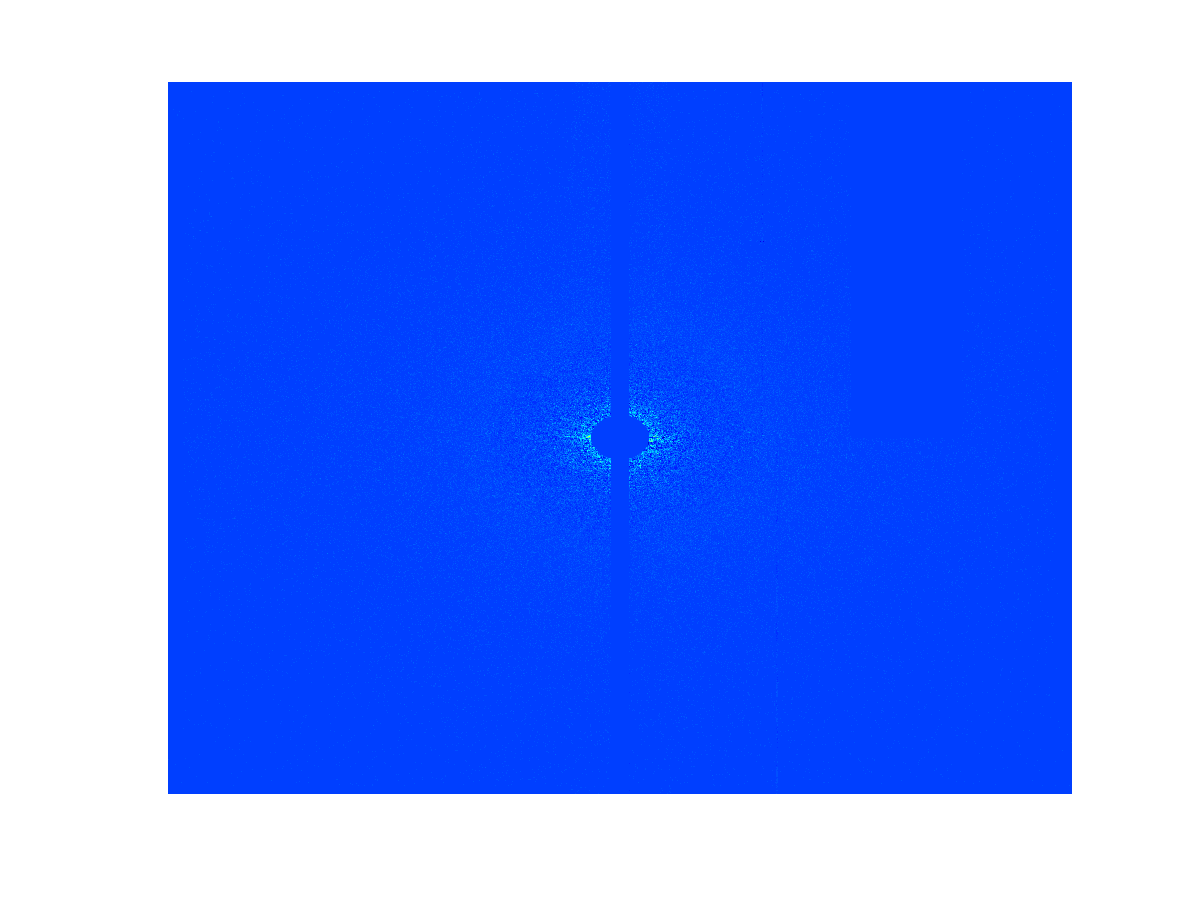
\includegraphics[width=.8\textwidth]{bad6}
\end{subfigure}
\caption{Diffraction patterns that does not contain strong scattering}
\label{fig:baddp2}
\end{figure}

After the selection of the good data was obtained, the next step was to obtain the value of each parameter in reciprocal space. To estimate the value of $dq$ (the step of reciprocal distance) for each pixel, following relation was used:
\begin{equation}
dq=\Delta_p/(\lambda Z)
\end{equation}
where $dq$ is reciprocal distance of a pixel in detector, 
$\Delta_p$ is length or size of a pixel in detector,
$\lambda$ is the wavelength used in experiment,
$Z$ is the distance from molecule to detector.
All those variables are given by this paper \cite{nanokassemeyer} where $\Delta_p=7.5\times 10^{-5}$ m, $Z=0.75$m, and $\lambda=10.38 $ \AA

After the quantity $dq$ for each pixel in detector grid was estimated, the next step was to do the interpolation from Cartesian grid into polar grid. The first step of interpolation was to specify or determine all point in polar grid. In this case, Shannon sampling was used for the radial step. The nanorice was estimated to have length 2000 \AA, therefore the radial step was $dq=1/(2D)=1/(4000) =2.5 \times 10^{-4}$ \AA. In addition to that, the angular step ($d\theta$) was taken as $2 \pi/360$. Figure \ref{fig:polargrid} show the arrangement of point in polar grid where $dq=2.5 \times 10^{-4} $  \AA and $d\theta=2 \pi/360$. 

\begin{figure}[ht]
  \centering
  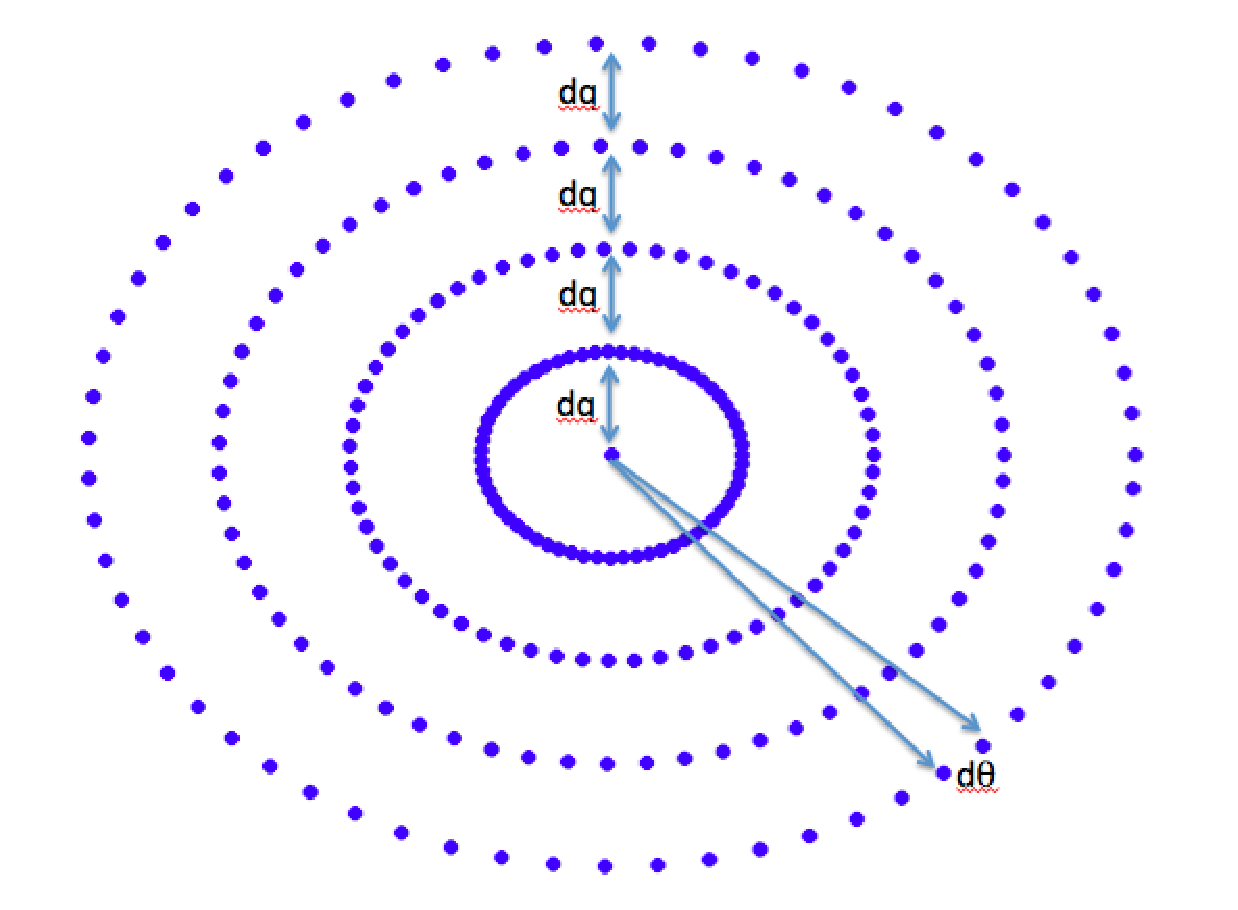
\includegraphics[width=.7\textwidth]{polargrid}
\caption{The point in polar coordinate}
\label{fig:polargrid}
\end{figure}

The scientific library in matlab was used to specify point in polar grid. The command in matlab to do the conversion is \textbf{pol2cart}. Below is an example of the code to specify point in polar grid:
\begin{lstlisting}[language=Octave]
//dq is the polar step in reciprocal space
// Nqp is the number of q point
dtheta=2*pi/360
qtheta=0:dtheta:2*pi-dtheta
qpolar=0:dq:dq*Nq          

// specify polar point in x-y form
[Xp,Yp]=pol2cart(qtheta,qpolar)  
\end{lstlisting}
The output of the code is the quantities $Xp$ and $Yp$. Those quantities represents the x-coordinate and y-coordinate of the polar grid. Thus, representation of polar grid in cartesian form can be calculated.  

The next step after determining the point in polar coordinate is to interpolate from Cartesian grid (detector grid) to polar coordinate where \Blq is defined. To get smooth function of estimation, cubic spline interpolation was used. The cubic spline interpolation divides each interval and approximates the point with third order polynomial. The polynomial is
\begin{equation}
f_{i}(x)=a_i + b_i x + c_i x^2 + d_i x^3
\label{eq:polycubspline}
\end{equation}
where subscript $i$ is the index of interval and $(a_i, b_i ,c_i , d_i)$ are the parameters needed to determined from boundary condition. The determination of the parameter used the following boundary condition:
\begin{align}
\begin{split}
f_{i}(x_{i-1})&=y_{i-1} \quad f_{i}(x_{i})=y_i \quad ,i=1,...,n \\
f'_{i}(x_i)&=f'_{i+1}(x_i) \quad i=1,...,n-1 \\
f''_{i}(x_i)&=f''_{i+1}(x_i) \quad i=1,...,n-1 
\end{split}
\label{eq:splinecond}
\end{align}  
where $y_i$ is the known function at $x_i$,  $f'_{i}(x_i)$ is the first derivative of the function and $f''_{i}(x_i)$ is the second derivative of the function. Additional two equations are needed to solve the parameters, which are called 'not-a-knot' condition. It impose condition of third derivative to be continous at two end point. Mathematically it is described as:
\begin{align}
\begin{split}
f'''_{1}(x_0)&=f'''_{2}(x_0) \quad i=1,...,n-1  \\
f'''_{n-2}(x_n)&=f'''_{n-1}(x_n) \quad i=1,...,n-1.   
\end{split}
\label{eq:splinecond2}
\end{align}
By applying the condition in equation \ref{eq:splinecond} and \ref{eq:splinecond2}, the parameters $(a_i, b_i ,c_i , d_i)$ in equation \ref{eq:polycubspline} can be found. Thus the value of the function in any point can be estimated by equation \ref{eq:polycubspline}. An example of the full derivation of the parameters is given in appendix \ref{ch:cubicspline}.  

The conversion of point in polar grid from Cartesian grid requires two dimensional interpolation. The extension from one dimensional to two dimensional is to approximate using two dimensional polynomial. The two dimensional polynomial is
\begin{equation}
f(x,y)=\sum_{i=0}^{3} \sum_{j=0}^{3} a_{ij} x^{i} y^{j}.
\label{eq:spline2d}
\end{equation}
Similar as before, coefficients $a_{ij}$ are determined from boundary condition in each interval ($i=1,...,n$),
\begin{align}
 f_{i}(x_i,y_i)=z(x_i,y_i) \quad  f_{i}(x_{i+1},y_i)=z(x_{i+1},y_i)  \\
 f_{i}(x_i,y_{i+1})=z(x_i,y_{i+1}) \quad  f_{i}(x_{i+1},y_{i+1})=z(x_{i+1},y_{i+1}) 
\end{align}
where $z(x_i,y_i)$ is the known function at $(x_i,y_i)$, the first derivative boundary
\begin{align}
&\frac{\partial f_{i}}{\partial x}\Bigr|_{x_i,y_i}=\frac{\partial f_{i+1}}{\partial x}\Bigr|_{x_i,y_i} \qquad 
\frac{\partial f_{i}}{\partial x}\Bigr|_{x_{i+1},y_i}=\frac{\partial f_{i+1}}{\partial x}\Bigr|_{x_{i+1},y_i} \\
&\frac{\partial f_{i}}{\partial x}\Bigr|_{x_i,y_{i+1}}=\frac{\partial f_{i+1}}{\partial x}\Bigr|_{x_i,y_{i+1}} \qquad 
\frac{\partial f_{i}}{\partial x}\Bigr|_{x_{i+1},y_{i+1}}=\frac{\partial f_{i+1}}{\partial x}\Bigr|_{x_{i+1},y_{i+1}} \\
&\frac{\partial f_{i}}{\partial y}\Bigr|_{x_i,y_i}=\frac{\partial f_{i+1}}{\partial y}\Bigr|_{x_i,y_i} \qquad 
\frac{\partial f_{i}}{\partial y}\Bigr|_{x_{i+1},y_i}=\frac{\partial f_{i+1}}{\partial y}\Bigr|_{x_{i+1},y_i} \\
&\frac{\partial f_{i}}{\partial y}\Bigr|_{x_i,y_{i+1}}=\frac{\partial f_{i+1}}{\partial y}\Bigr|_{x_i,y_{i+1}} \qquad 
\frac{\partial f_{i}}{\partial y}\Bigr|_{x_{i+1},y_{i+1}}=\frac{\partial f_{i+1}}{\partial y}\Bigr|_{x_{i+1},y_{i+1}} 
\end{align}
with the second derivative boundary,
\begin{align}
&\frac{\partial^2 f_{i}}{\partial x\partial y}\Bigr|_{x_i,y_i}=\frac{\partial^2 f_{i+1}}{\partial x \partial y}\Bigr|_{x_i,y_i} \qquad 
\frac{\partial^2 f_{i}}{\partial x\partial y}\Bigr|_{x_{i+1},y_i}=\frac{\partial^2 f_{i+1}}{\partial x \partial y}\Bigr|_{x_{i+1},y_i} \\
&\frac{\partial^2 f_{i}}{\partial x \partial y}\Bigr|_{x_i,y_{i+1}}=\frac{\partial^2 f_{i+1}}{\partial x \partial y}\Bigr|_{x_i,y_{i+1}} \qquad 
\frac{\partial^2 f_{i}}{\partial x \partial y}\Bigr|_{x_{i+1},y_{i+1}}=\frac{\partial^2 f_{i+1}}{\partial x \partial y}\Bigr|_{x_{i+1},y_{i+1}} \\
\end{align}


By applying the condition of continuty in the function, the first derivative and the second derivative, the parameter $a_{i,j}$ can determined in equation \label{eq:spline2d}. Thus, the value of the function in any point can be estimated by equation \ref{eq:spline2d}. 

The derivation to calculate the parameters in two dimension interpolation can be complicated. However, there are available several scientific libraries to calculate cubic spline interpolation. The library that I used to convert Cartesian grid into polar grid was matlab libray under the command \textbf{interp2}. A snippet of the code to use \textbf{interp2} is shown below:
\begin{lstlisting}[language=Octave]
//dqc is the reciprocal distance per pixel
// N is the number of pixel in one dimension divided by 2
[Xc,Yc]=meshgrid(-N*dqc:dqc:N*dqc,-N*dqc:dqc:N*dqc)                                        

//dq is the polar step in reciprocal space
// Nqp is the number of q point
dtheta=2*pi/360
qtheta=0:dtheta:2*pi-dtheta
qpolar=0:dq:dq*Nq          

// specify the polar point in x-y form
[Xp,Yp]=pol2cart(qtheta,qpolar)  

//Do the interpolation 
// F is the known value in each cartesian point
// V is the diffraction pattern in polar point
V=interp2(Xc,Yc,F,Xp,Yp,'spline')
\end{lstlisting}
The output of the code is the quantity $V$ where it hold the value of interpolation in polar grid. Thus, a set of new polar diffraction patterns can be obtained with the cubic spline interpolation. 

After the diffraction patterns were sampled in polar point, the calculation of the angular pair correlation can be done. The pair correlation do the sum over all diffraction patterns and correlate them in angularly. Formula in equation \ref{eq:crosscor} was used to calculate $C_{2}$ where  $I(q,\phi)$ is the diffraction pattern in polar grid and $(q,\phi)$ are the point in polar grid. Subsequent to that, \Blq was calulated using matrix inversion in equation \ref{C2definition}. As a result of that, \Blq from the experiment data of nanorice could be determined.   

It is important to note that, the derivation to get \Blq from equation \ref{eq:crosscor} to equation \ref{C2definition} use fundamental assumption where all random angle span through all possible angle (equation \ref{eq:orthotheorem}). However, there are only 200 good diffraction patterns available from the experimental data. That is why it is important to check the convergence of \Blq from 200 diffraction patterns.    

The matrices \Blq were calculated from 200 diffraction patterns of nanorice. Subsequent to that, SVD on the \Blq was performed for each $l$ and its nonzero singular value is displayed in figure \ref{fig:svdnanoexp}

It is shown in the plot that all the matrices \Blq, which correspond to $l$, have singular values more than $2l+1$. In other words, the plot shows the behavior more asymmetric than an asymmetric pattern, which is not plausible. The only explanation is that the \Blq is not in the form of dot product. As explained earlier, if \Blq is a form of dot product then the SVD on \Blq will have singular values less than or equal to the asymmetric pattern, which is $2l+1$. In conclusion, the \Blq calculated from 200 diffraction pattern of nanorice doesn't converge to its theoritical value. 

\begin{figure}[h!]
  \centering
  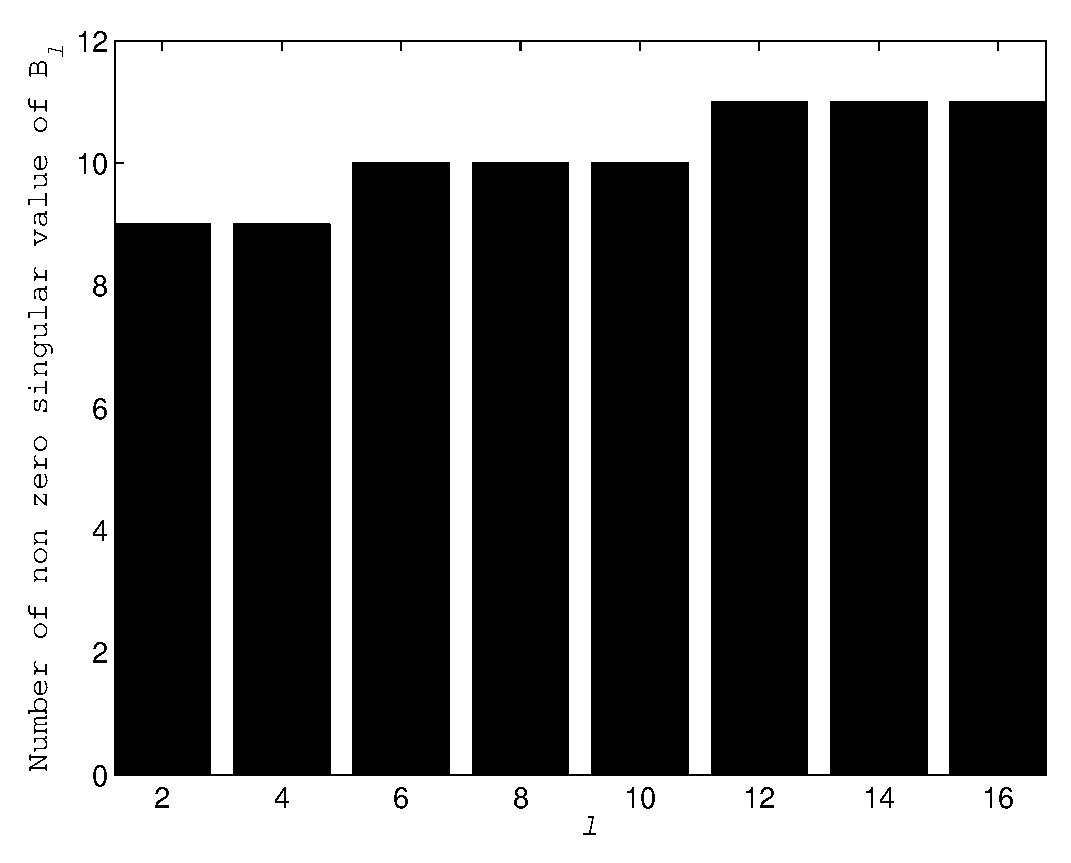
\includegraphics[width=.8\textwidth]{svdBnanoexp}
\caption{The number of nonzero singular value is more than $2 l+1$. The data doesn't show the convergence of \Blq}
\label{fig:svdnanoexp}
\end{figure}

Before using the \Blq for structure determination, checking accurate convergence is priority. Here one way to check the convergence is known by using SVD on the \Blq. If it is found than the number of singular values of \Blq is higher than those from asymmetric pattern then additional steps to correct the \Blq is needed. 

